\def\year{2015}
%File: formatting-instruction.tex
\documentclass[letterpaper]{article}
\usepackage{aaai}
\usepackage{times}
\usepackage{helvet}
\usepackage{courier}
\usepackage{graphicx}
\usepackage{subcaption}
\usepackage{}
\frenchspacing
\setlength{\pdfpagewidth}{8.5in}
\setlength{\pdfpageheight}{11in}
\pdfinfo{
/Title (Insert Your Title Here)
/Author (Put All Your Authors Here, Separated by Commas)}
\setcounter{secnumdepth}{0}  
 \begin{document}
% The file aaai.sty is the style file for AAAI Press 
% proceedings, working notes, and technical reports.
%
\title{Combining Learning and Evolution in OpenNERO}
\author{Jacob Robertson \and Yun Wu\\
Department of Computer Science\\
University of Texas at Austin\\
}
\maketitle
\begin{abstract}
\begin{quote}
AAAI
\end{quote}
\end{abstract}

\section{Experiments and Results}
In this paper, we evaluate our rtNEAT+Q algorithm in OpenNERO\footnote{https://code.google.com/p/opennero/}. OpenNERO is an open source software platform designed for research and education in Artificial Intelligence. The project is based on the Neuro-Evolving Robotic Operatives (NERO) game developed by graduate and undergraduate students at the Neural Networks Research Group and Department of Computer Science at the University of Texas at Austin. In the NERO game, The learning agents in NERO are simulated robots, and the goal is to train a team of these agents for combat. The agents begin the game with no skills and only the ability to learn. We tested the algorithm in different tasks and compare its performance to that of rtNEAT and Q-learning.

\subsection{Approaching a flag}
The first task is to train the agents running towards a flag. The distance between the spawn spot of agents and the flag is 141.4. Figure~\ref{fig:flag} illustrates the result. The green line is the average distance among all the agents and the blue line shows the minimum distance. From Figure~\ref{fig:flag_q} we can find that the result of Q learning in continuous domain is quite unstable. Also, rtNEAT, on the other hand, performs much better. Agents get to the flag pretty quick (around 25 ticks). The average distance converges at around 200 ticks when almost all the agents has learnt to approach a flag. The combination of rtNEAT and Q learning has similar performance with rtNEAT. It converges quickly but the average distance is longer than rtNEAT alone. 
\begin{figure*}[ht]
\centering
\begin{subfigure}{0.7\columnwidth}
  \centering
  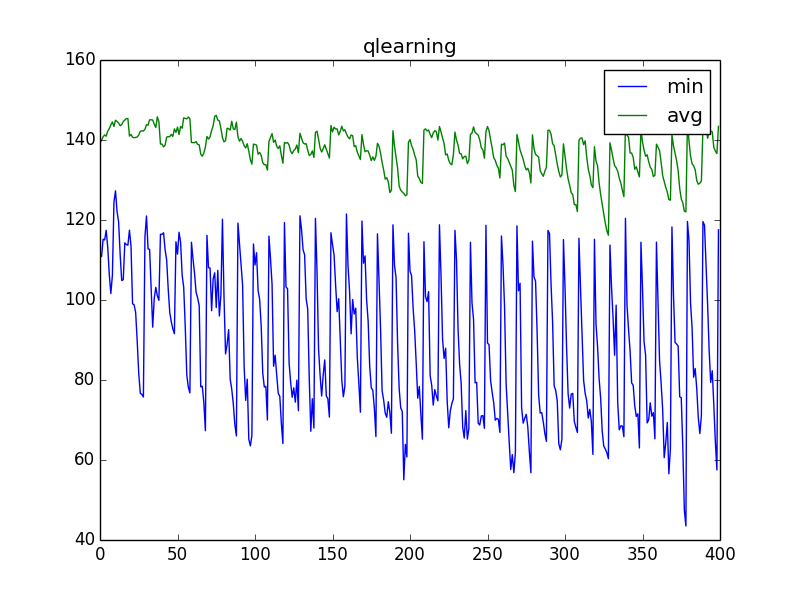
\includegraphics[width=\columnwidth]{flag_qlearning.png}
  \caption{Q Learning}
  \label{fig:flag_q}
\end{subfigure}%
\begin{subfigure}{0.7\columnwidth}
  \centering
  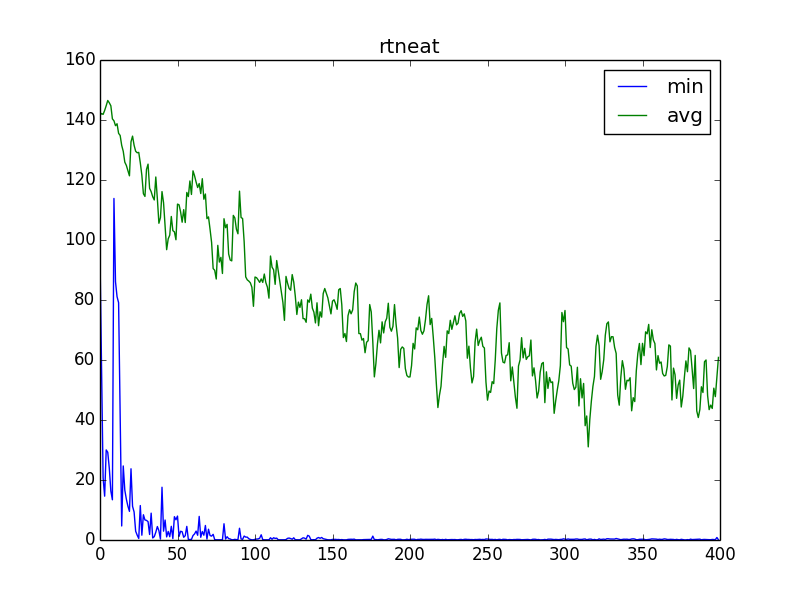
\includegraphics[width=\columnwidth]{flag_rtneat.png}
  \caption{rtNEAT}
  \label{fig:flag_neat}
\end{subfigure}
\begin{subfigure}{0.7\columnwidth}
  \centering
  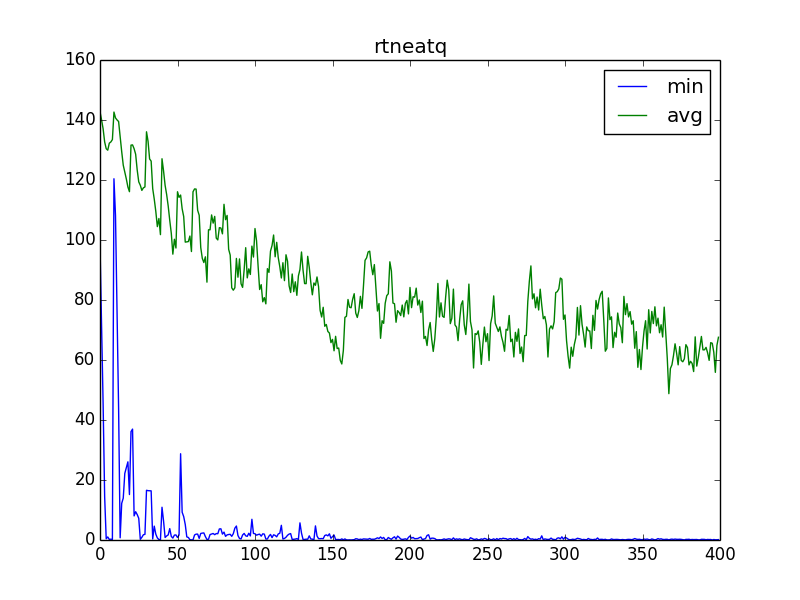
\includegraphics[width=\columnwidth]{flag_rtneatq.png}
  \caption{rtNEAT + Q Learning}
  \label{fig:flag_neatq}
\end{subfigure}
\caption{Approaching a flag}
\label{fig:flag}
\end{figure*}

\subsection{Approaching a moving flag}


\subsection{Approaching a flag with obstacles}
However, when it comes to more complex tasks, the benefit of learning appears. In the third experiments, the distance between agents and the flag is 267. And there is a wall with width 100 between them. Agents need to learn to get around the wall to approach the flag. The result is in Figure~\ref{fig:wall}. Within 700 ticks, Q learning agents never get a chance to get close to the flag. From Figure~\ref{fig:wall_neat} and Figure~\ref{fig:wall_neatq}, it is clear that at first, agents learn to go directly towards flag until they are blocked by the wall. Then exploration then helps find the way around. Q learning then back propagate their network and learn the route. Finally, although rtNEAT+Q converges more slowly than rtNEAT, agents runs toward the flag more fast. The average distance of rtNEAT converges at 180 while that of rtNEAT+Q at 150. 

Here is the reason why rtNEAT+Q benefits complex tasks. As shown in previous section, rtNEAT+Q take advantage of TD updates to tune parameters of neural network. However, Q learning needs time to learn. In simple task, structure of neural network is relatively simple. rtNEAT itself is able to evolve the optimal method quickly. However, for complicated tasks, it takes more time for evolution. In the mean time, Q learning is able to back propagate the network based on TD updates. Larmerkian system is used in our implementation, where the result of learning is kept to the next generation. 
\begin{figure*}[ht]
\centering
\begin{subfigure}{0.7\columnwidth}
  \centering
  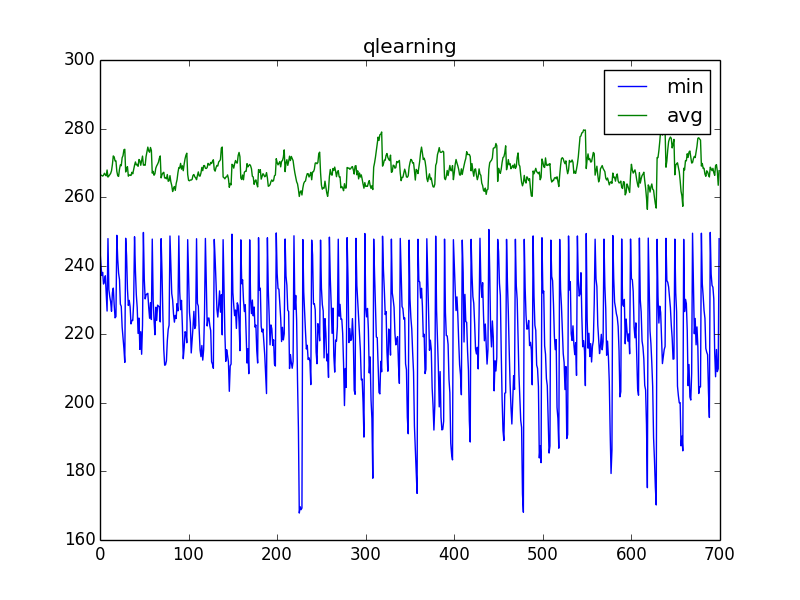
\includegraphics[width=\columnwidth]{wall_qlearning.png}
  \caption{Q Learning}
  \label{fig:wall_q}
\end{subfigure}%
\begin{subfigure}{0.7\columnwidth}
  \centering
  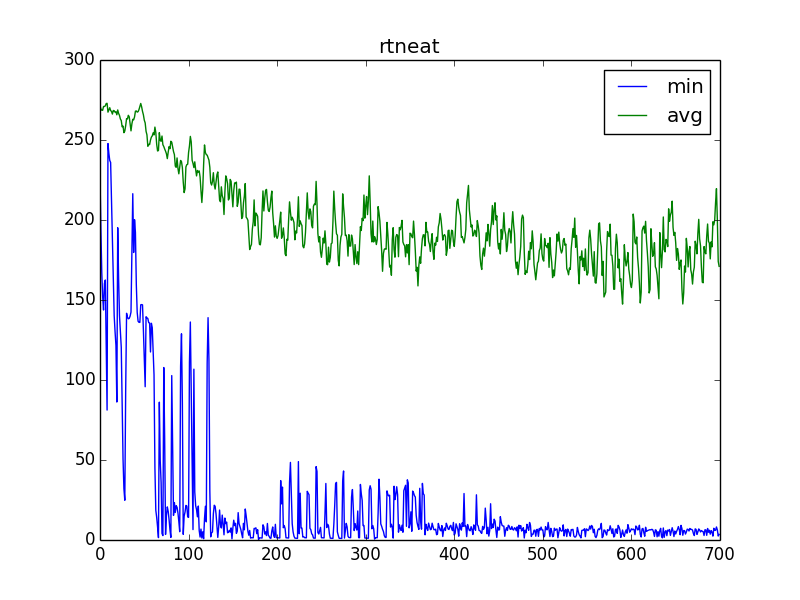
\includegraphics[width=\columnwidth]{wall_rtneat.png}
  \caption{rtNEAT}
  \label{fig:wall_neat}
\end{subfigure}
\begin{subfigure}{0.7\columnwidth}
  \centering
  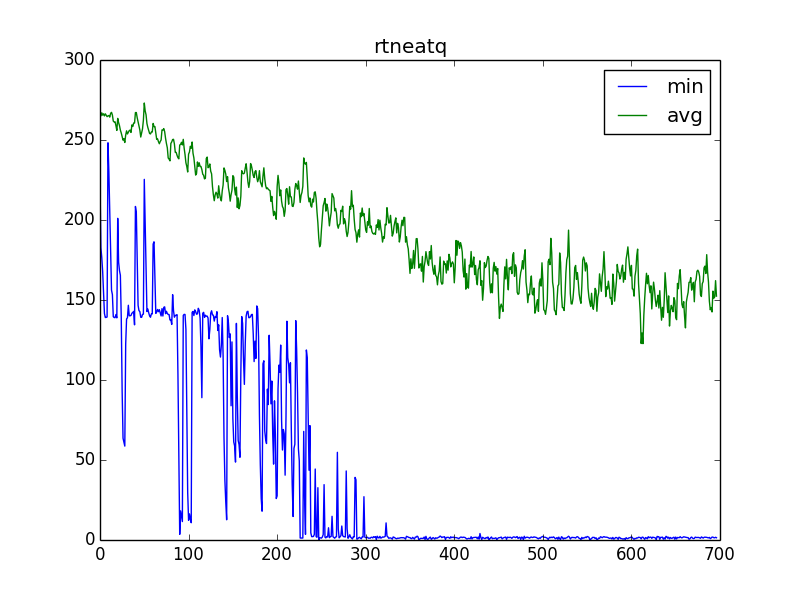
\includegraphics[width=\columnwidth]{wall_rtneatq.png}
  \caption{rtNEAT + Q Learning}
  \label{fig:wall_neatq}
\end{subfigure}
\caption{Approaching a flag with obstacles}
\label{fig:wall}
\end{figure*}


\end{document}
